\chapter{Análisis de conjunto de datos transcripcionales Wiegel}
En este capítulo analizaremos el conjunto de datos transcripcionales Wiegel \& Lohmann para la planta Arabidopsis thaliana presentados en la sección \ref{sec:wiegel}, utilizando para ello los métodos de agrupamiento k-means (sección \ref{sec:agrupamientos_no_jerarquicos}) y corte de árbol dinámico híbrido (sección \ref{sec:grupos_en_agrupamiento_jerarquico}) introducidos en el capítulo \ref{materiales_y_metodos} para obtener grupos en el espacio de expresión.\\
Una vez obtenidos los grupos en el espacio de expresión, utilizaremos los índices BHI e Interacting Densities para cuantificar el grado de coherencia entre estas estructuras y los conocimientos (entendidos como nociones de similitud) en el espacio GO.\\
Luego, analizaremos la coherencia de los resultados obtenidos en el espacio de expresión con la de resultados obtenidos en otros espacios de conocimiento, como GO (sección \ref{sec:go}), PIN  (sección \ref{sec:redes}) y KEGG (sección \ref{sec:kegg}), esperando que estos conocimientos sean diferentes pero no ortogonales, utilizando para ello el índice KTA. 

\section{Descripción del dataset}
\hl{esto esta en sec:wiegel habra que profundizar mas?}
\section{Métricas transcripcionales}
\hl{esto esta en el capitulo 3, o la idea es poner otra cosa?}
\section{Agrupamiento}

\subsection{Proceso de filtrado}
El conjunto de datos Wiegel utilizado consta de los niveles de expresión de 22810 sondas que se mapean a 20149 genes a lo largo de 11 tratamientos diferentes y con entre 4 y 9 muestreos en dos réplicas. Para poder manejar esta cantidad de información es necesario realizar un filtrado (una selección) previo de los datos que permita quedarse únicamente con aquellos genes que se expresaron o inhibieron, ya que serán estos los genes que estarán siendo regulados en función del tratamiento y por lo tanto los de interés.\\
Para ello, se aplicaron dos tipos de filtros por tratamiento, por desviación estandar y por de tipo ``$K sobre A$''. Para el primero, se calculó la desviación estandar por gen a lo largo de todo el tratamiento y se decidió tomar los genes cuya desviación estandar se encontrara en el cuantil 0.9, es decir, utilizar el 10\% de los genes con mayor desviación estandar, considerando estos como los que formaron parte de la respuesta biológica al tratamiento. La figura \ref{fig:densidad_de_desviacion_estandar} muestra la distribución de probabilidad acumulada (empírica) de la desviación estandar para los genes del tratamiento ``Cold''.\\
Una vez aplicado este filtro por desviación estandar, se aplicó un filtro de tipo ``$K sobre A$'', que toma unicamente con aquellos genes que tengan al menos $K$ datos por encima del valor $A$. En nuestro caso, decidimos utilizar como valor de $K$, la mitad de las mediciones que tuviera el tratamiento. Si el tratamiento tenía mediciones cada 0 minutos, 30 minutos, 1 hora, 3 horas, 6 horas, 12 horas y 24, es decir, 6 mediciones en total, se tomó $K = 3$. Para $A$, se decidió utilizar una medida usual de $A=4$, ya que valores de señal menores a $4$ no se distinguen del ruido \hl{paper sobre esto? cuales son las unidades de estos datos? son en escala logaritmica?}. La figura \ref{fig:densidad_para_niveles} muestra la distribución de probabilidad para los niveles de expresión para el tratamiento ``Cold''.
\begin{figure*}[t!]
    \centering
    \begin{subfigure}[t]{0.4\textwidth}
    \centering
    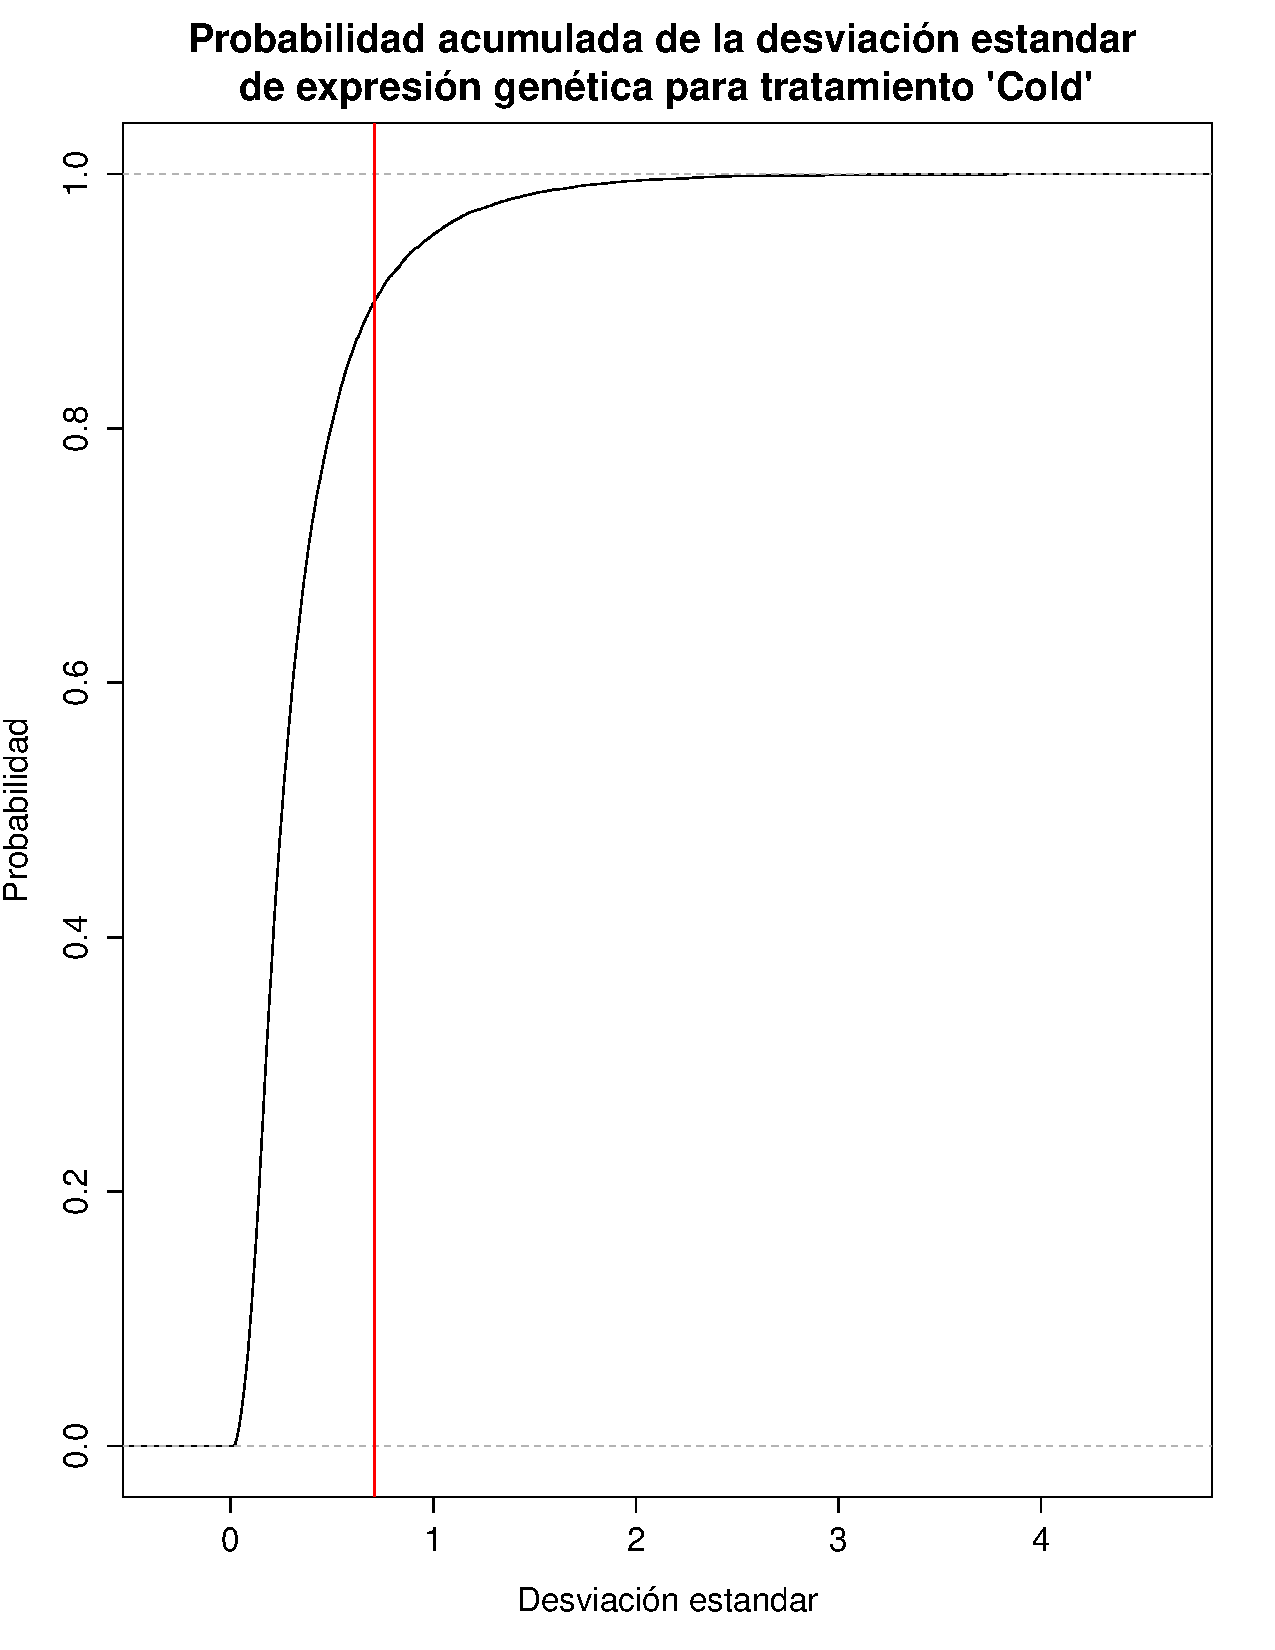
\includegraphics[width=1\textwidth]{densidad_de_desviacion_estandar}
    \caption{Distribución de probabilidad acumulada de la desviación estandar para los genes del tratamiento \textit{Cold}. Todos los genes con desviación estandar menor que la indicada por la recta vertical roja son descartados.}
    \label{fig:densidad_de_desviacion_estandar}
    \end{subfigure}
    \begin{subfigure}[t]{0.4\textwidth}
    \centering
    \includegraphics[width=1\textwidth]{densidad_para_niveles}
    \caption{distribución de probabilidad para los niveles de expresión para el tratamiento \textit{Cold}. La recta vertical roja muestra el valor a partir del cual se hace un corte.}
    \label{fig:densidad_para_niveles}
    \end{subfigure}
    \caption{Funciones de distribución de probabilidad para perfiles de expresión}
\end{figure*}
La tabla \ref{tabla:genes_por_tratamiento} muestra los filtros aplicados y la cantidad de genes finales por tratamiento.
Una vez aplicados los filtros y obtenido los genes de mayor variabilidad en su expresión, se estandarizaron los datos obtenidos para poner a todos los genes en igualdad de condiciones y pesarlos de la misma forma en el agrupamiento. Un procedimiento normal de estandarización de genes para que cada gen tenga media cero y varianza unitaria implica realizar la transformación:
\begin{equation}
	\tilde{x_i} = \frac{x_i-\bar{x}}{s_x}
\end{equation}
Con $x_i$ cada observación del gen $x$ a lo largo del tiempo para un determinado tratamiento. Una vez realizado el filtrado y estandarizado procedimos a agrupar los datos mediante los diferentes métodos mencionados en el capítulo 3.
\begin{table}[t]
  \centering
\begin{tabular}{| l | c | c | c |}
\hline
Tratamiento & $\sigma$ & A & Cantidad de genes \\
\hline
Control & 0.37 & 4 & 1885 \\
\hline
Frío & 0.71 & 3 & 1955 \\
\hline
Osmótico & 0.71 & 3 & 1923 \\
\hline
Sal & 0.88 & 3 & 1927 \\
\hline
Sequía & 0.54 & 4 & 1870 \\
\hline
Genotóxico & 0.46 & 3 & 1899 \\
\hline
Oxidativo & 0.41 & 3 & 1880 \\
\hline
UV-B & 0.51 & 4 & 1872 \\
\hline
Heridas & 0.41 & 4 & 1877 \\
\hline
Calor & 0.75 & 2 & 1960 \\
\hline
Calor y recuperación & 0.65 & 2 & 1944 \\
\hline                                         
\end{tabular}
\caption{Cantidad de genes y filtros utilizados por tratamiento.}
\label{tab:genes_por_tratamiento}
\end{table}
\subsection{Agrupamiento con k-means}
El método de agrupamiento k-means hace uso de la distancia euclidia para minimizar la suma de los cuadrados. Si los datos están estandarizados y centrados, es posible relacionar la distancia euclidia $d$ con el coeficiente de correlación mediante la fórmula:
\begin{equation}
	d(\vec{x}, \vec{y}) = \sqrt{2(d-1)(1-r(\vec{x}, \vec{y}))}
\end{equation}
y por lo tanto, para datos estandarizados, la distancia euclidia se comportará de forma similar a la distancia de correlación y podremos utilizar el método k-means. \hl{revisar esta frase y que quiero decir}\\
Para decidir el k a utilizar en el método, se realizó un barrido variando k entre $k=2$ y $k=30$ con pasos de 1. Al tratarse de un método heurístico, no existe garantía de convergencia al óptimo global y el resultado del mismo puede entonces depender de los grupos iniciales. Por lo tanto, para cada k, se realizaron cien agrupamientos y se midieron los índices de validación internos Calinski-Harabasz y Dunn en cada uno, definidos respectivamente como:
\begin{equation}
	CH_k = \frac{SS_B}{SS_W}\frac{n-k}{n-1}
\end{equation}
con $SS_B$ el promedio de la varianza entre grupos, $SS_W$ el promedio de la varianza intra grupos, k es el número de grupos y n el número de observaciones y:
\begin{equation}
	DI = \frac{min\delta}{\max\Delta}
\end{equation}
con $\delta$ la menor de las de distancias entre grupos y $\Delta$ la mayor de las distancias intra grupos.\\
Grupos bien definidos tendrán distancias grandes entre ellos comparados con las distancias intra grupos, por lo que a mayor $CH$ o $DI$, mejor definidos estarán los grupos.\\
Las figuras \ref{fig:barrido_k_ch} y \ref{fig:barrido_k_dunn} muestran un gráfico de caja (o boxplot en inglés), para el índice CH y Dunn respectivamente para cada uno de los k en el barrido. Un boxplot consiste en una caja con una linea horizontal que indica el segundo cuartil, es decir, la mediana del conjunto de datos, y dos lineas verticales llamadas bigotes (o whiskers en inglés) que se extiende una desde el primer cuartil hasta el valor más pequeño del conjunto (con excepción de puntos aislados) y la otra desde el tercer cuartil hasta el valor más grande. Los puntos aislados se grafican de forma separada en el gráfico.
\begin{figure*}[t!]
    \centering
    \begin{subfigure}[t]{0.45\textwidth}
    \centering
    \includegraphics[width=1\textwidth]{barrido_k_ch}
    \caption{Índice CH de particiones realizadas con k-means para k entre 2 y 30.}
    \label{fig:barrido_k_ch}
    \end{subfigure}
    \begin{subfigure}[t]{0.45\textwidth}
    \centering
    \includegraphics[width=1\textwidth]{barrido_k_dunn}
    \caption{Índice Dunn de particiones realizadas con k-means para k entre 2 y 30.}
    \label{fig:barrido_k_dunn}
    \end{subfigure}
    \caption{Índices de validación interna para particiones realizadas con k-means}
\end{figure*}
Se observa que la cantidad de grupos que maximiza estos índices es 2. Se realizó entonces un agrupamiento con $k=2$, obteniéndose los perfiles que muestra la figura \ref{fig:perfiles_k_means}, con una correlación media de $\rho=0.74$ para el primero y de  $\rho=0.79$ para el segundo, con aproximadamente el 50\% de los genes en cada grupo.
\begin{figure}[h]
    \centering
    \includegraphics[width=0.8\textwidth]{perfiles_k_means}
    \caption{Perfiles de expresión génica obtenidos con el método k-means (k=2) para el tratamiento 'Frío'. En azul, el valor medio de cada grupo.}
    \label{fig:perfiles_k_means}
\end{figure}
Estas estructuras tan grandes son de difícil interpretación biológica, ya que si bien las respuestas de expresión dentro de cada grupo son similares, existe mucha heterogeneidad en las funciones biológicas de los genes que los componen. El método k-means está entonces trabajando a una escala que no permite extraer información biológica de los grupos. Será necesario entonces aumentar la granularidad mediante otros métodos de agrupamiento.
\subsection{Agrupamiento con corte de árbol dinámico}
Utilizando el método de corte de árbol dinámico se realizó para cada tratamiento 
\hl{ideas: poner aca que se probo con deepsplit 1 y deepsplit 4. Que se logra meter mucho mejor, mostrar algunos perfiles para algun tratamiento para ambos y mostrar quizas una tabla con cada tratamiento cuantos clusters y que tamanios. charlar de nuevo sobre la escala.}
\subsection{Análisis de los métodos y problemas de escala de resolución}

\section{Coherencia entre la métrica transcripcional y otros espacios de conocimiento}
\hl{idea esperamos que los conocimientos (entendidos como nociones de similitud) de los distintos espacios sean diferentes pero no ortogonales...cuantificacion...veamos que estructuras son en cierto grado coherentes}
\subsection{Interacting densities}
\hl{genex1 /genex4  VS BPa/BPb/CC}
\hl{PINinfomap / KEGGinfomap/LCI para referencia}
\subsection{KTA y zKTA}
\hl{Global}
\hl{KTA Genex por tratamiento + PIN + KEGG + LCI / GOBPa, GOBPb, GOCC}
\hl{zKTA: por tratamiento Gx/GOBPa, Gx/GOBPb, Gx/GOCC, Gx/PIN, Gx/LCI, Gx/Kegg}